\chapter{Results}
\label{chapter:results}
In this chapter we will look at the results of the experiments discussed in chapter~\ref{chapter:experiments}.

\Crefrange{tab:d1}{tab:d4} show the ratio of articles which resulted in no new words, no new pairs or both. In the cases where filtering was applied a shorthand for the filter type (cf=collection frequency, tf=term frequency) is included as well as the threshold. We noted that filtering did in fact increase the number of empty output-sets of either size and in the cases of the collection frequency and term frequency filters along with any pre-enumeration filtering (Configuration-3) the change was quite drastic.

\begin{center}
\begin{table}
  \begin{tabular}{|l|c|c|c|}
    \hline
    &  No new words & No new Pairs & Both \\ \hline
    Configuration-1                    & 0.04  & 0.03  & 0.01 \\ \hline
    Configuration-2 (cf: 5)            & 0.00  & 1.00  & 0.93 \\ \hline
    Configuration-2 (tf: 5)            & 0.58  & 0.42  & 0.41 \\ \hline
    Configuration-2 (tfidf: 5)         & 0.05  & 0.35  & 0.01 \\ \hline
    Configuration-3 (cf: 5)            & 0.19  & 0.92  & 0.85 \\ \hline
    Configuration-3 (tf: 5)            & 0.01  & 0.99  & 0.96 \\ \hline
    Configuration-3 (tfidf: 5)         & 0.00  & 0.74  & 0.01 \\ \hline
    Configuration-4                    & 0.04  & 0.03  & 0.01 \\ \hline
    Configuration-4 (tfidf: 5)         & 0.04  & 0.52  & 0.02 \\ \hline
  \end{tabular}
  \caption{The outcomes from running different configurations on dataset D1}
  \label{tab:d1}
\end{table}
\end{center}

\begin{center}
\begin{table}
  \begin{tabular}{|l|c|c|c|}
    \hline
    &  No new words & No new Pairs & Both \\ \hline
    Configuration-1                    & 0.10  & 0.01  & 0.00 \\ \hline
    Configuration-2 (tfidf: 5)         & 0.12  & 0.25  & 0.00 \\ \hline
    Configuration-3 (tfidf: 5)         & 0.01  & 0.69  & 0.00 \\ \hline
    Configuration-4                    & 0.10  & 0.01  & 0.00 \\ \hline
    Configuration-4 (tfidf: 5)         & 0.11  & 0.36  & 0.01 \\ \hline
  \end{tabular}
  \caption{The outcomes from running different configurations on dataset D2}
  \label{tab:d2}
\end{table}
\end{center}

\begin{center}
\begin{table}
  \begin{tabular}{|l|c|c|c|}
    \hline
    &  No new words & No new Pairs & Both \\ \hline
    Configuration-1                    & 0.16  & 0.10  & 0.01 \\ \hline
    Configuration-2 (tfidf: 5)         & 0.16  & 0.30  & 0.01 \\ \hline
    Configuration-3 (tfidf: 5)         & 0.11  & 0.55  & 0.01 \\ \hline
    Configuration-4                    & 0.16  & 0.10  & 0.01 \\ \hline
    Configuration-4 (tfidf: 5)         & 0.16  & 0.32  & 0.01 \\ \hline
  \end{tabular}
  \caption{The outcomes from running different configurations on dataset D3}
  \label{tab:d3}
\end{table}
\end{center}

\begin{center}
\begin{table}
  \begin{tabular}{|l|c|c|c|}
    \hline
    &  No new words & No new Pairs & Both \\ \hline
    Configuration-1                    & 0.13  & 0.74  & 0.13 \\ \hline
    Configuration-2 (tfidf: 5)         & 0.23  & 0.74  & 0.65 \\ \hline
    Configuration-3 (tfidf: 5)         & 0.18  & 0.65  & 0.33 \\ \hline
    Configuration-4                    & 0.18  & 0.64  & 0.08 \\ \hline
    Configuration-4 (tfidf: 5)         & 0.32  & 0.64  & 0.55 \\ \hline
  \end{tabular}
  \caption{The outcomes from running different configurations on dataset D4}
  \label{tab:d4}
\end{table}
\end{center}

One of the events touched upon in the D2 dataset is the BP-oil spill in the Gulf of Mexico\footnote{\url{https://en.wikipedia.org/wiki/Deepwater_Horizon_oil_spill}} and president Obama's actions revolving that incident. \Crefrange{lst:original}{lst:config6} show the enumerations of an article in which the event was mentioned for the second time, enumerated using different configurations. In this case the event would be that president Obama answered questions regarding the oil spill.

As is to be expected, the enumerations using Configuration-2 and Configuration-4 are very similar since most of the articles in the dataset only contain one sentence and therefore only one sub-bag. Apart from the enumeration generated by Configuration-3 which contains no useful insights about the contents of the article, the generated enumerations appear to capture the main gist of the article. For configurations 1,3 and 4 the minimal new sets have been sorted based on TF-IDF score, in descending order. 

%In \cref{tab:nodeCounts} we show the number of different new pairs in which the involved words occurred. We observe that in this case words which appear in many new pairs appear to have high significance within the article.

\begin{lstlisting}[frame=single,
    caption=Original text,
    label={lst:original},
  ]
  May 27  – President Obama holds a news conference in the East Room to answer questions about the  BP  Deepwater Horizon  Gulf of Mexico oil spill . 
\end{lstlisting}

\begin{lstlisting}[frame=single,
    caption=Configuration-1,
    label={lst:config1},
  ]
New Words: {deepwat, horizon}
New Pairs: {(question, bp), (spill, question), (gulf, bp), (spill, answer), (bp, answer), (gulf, question), (gulf, spill), (question, news), (bp, news), (spill, news), (gulf, answer), (question, oil), (mexico, question), (mexico, bp), (mexico, spill), (spill, 27), (question, 27), (bp, 27), (answer, news), (gulf, news), (question, east), (bp, east), (spill, east), (bp, confer), (spill, confer), (question, confer), (question, room), (bp, room), (spill, room), (question, may), (spill, hold), (bp, hold), (question, hold), (oil, answer), (mexico, answer), (gulf, 27), (27, answer), (oil, news), (east, answer), (confer, answer), (gulf, confer), (room, answer), (gulf, room), (mexico, news), (gulf, may), (may, answer), (gulf, hold), (27, news), (east, news), (room, news), (may, news), (oil, 27), (confer, oil), (mexico, 27), (room, oil), (oil, hold), (mexico, confer), (east, 27), (mexico, room), (confer, 27), (mexico, hold), (room, 27), (27, may), (east, may)}
\end{lstlisting}

\begin{lstlisting}[frame=single,
    caption=Configuration-2,
    label={lst:config3},
  ]
New Words: {deepwat, horizon}
New Pairs: {(question, bp), (spill, question), (gulf, bp), (spill, answer), (bp, answer), (gulf, question), (gulf, spill), (question, news), (bp, news), (spill, news), (question, oil), (mexico, question), (mexico, bp), (mexico, spill), (spill, 27), (question, 27), (bp, 27), (question, east), (bp, east), (spill, east), (bp, confer), (spill, confer), (question, confer), (question, room), (bp, room), (spill, room), (question, may), (spill, hold), (bp, hold), (question, hold)}
\end{lstlisting}

\begin{lstlisting}[frame=single,
    caption=Configuration-3,
    label={lst:config5},
  ]
New Words: {horizon, deepwat, question}
  New Pairs: {}
\end{lstlisting}

\begin{lstlisting}[frame=single,
    caption=Configuration-4,
    label={lst:config6},
  ]
New Words: {deepwat, horizon}
New Pairs: {(question, bp), (spill, question), (gulf, bp), (spill, answer), (bp, answer), (gulf, question), (gulf, spill), (question, news), (bp, news), (spill, news), (question, oil), (mexico, question), (mexico, bp), (mexico, spill), (spill, 27), (question, 27), (bp, 27), (question, east), (bp, east), (spill, east), (bp, confer), (spill, confer), (question, confer), (question, room), (bp, room), (spill, room), (question, may), (spill, hold), (bp, hold), (question, hold), (question, –)}
\end{lstlisting}

\Crefrange{fig:setPlot1}{fig:setPlot4} show how the amount of minimal new sets of size less than 3 found in enumeration change over time using different configurations. In all cases the amount of new words found decreases over time while the amount of new pairs found tends to increase over time.

\begin{figure}[ht]
  \centering
  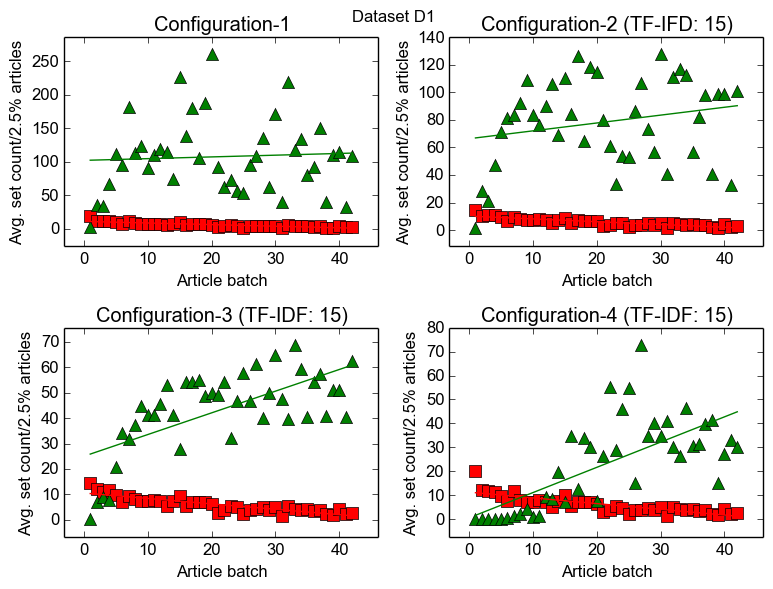
\includegraphics[scale=0.70]{images/D1-plot.png}
  \caption{Average number of new words and new pairs per batch of 2.5\% of all articles in dataset D1}
  \label{fig:setPlot1}
\end{figure}

\begin{figure}[ht]
  \centering
  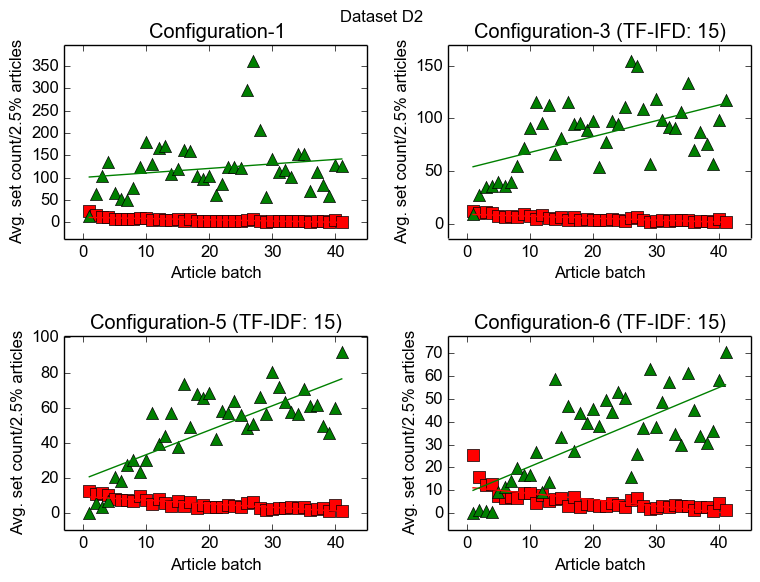
\includegraphics[scale=0.70]{images/D2-plot.png}
  \caption{Average number of new words and new pairs per batch of 2.5\% of all articles in dataset D2}
  \label{fig:setPlot2}
\end{figure}

\begin{figure}[ht]
  \centering
  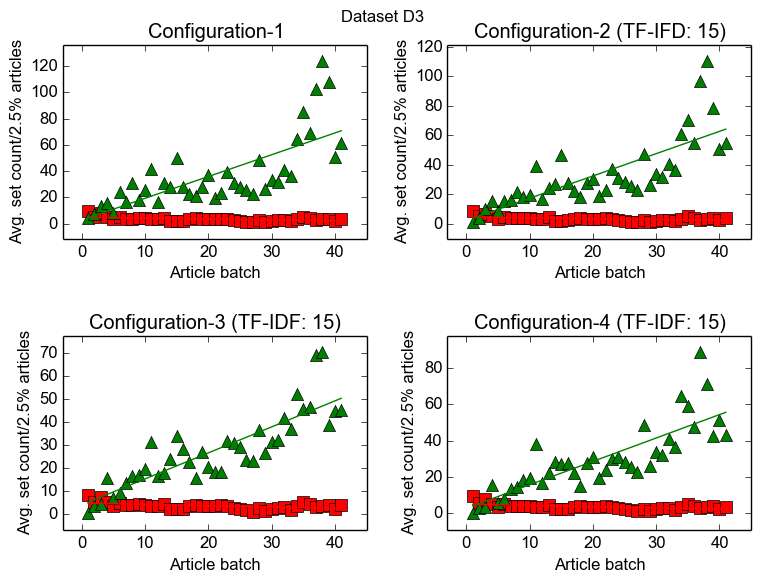
\includegraphics[scale=0.70]{images/D3-plot.png}
  \caption{Average number of new words and new pairs per batch of 2.5\% of all articles in dataset D3}
  \label{fig:setPlot3}
\end{figure}

\begin{figure}[ht]
  \centering
  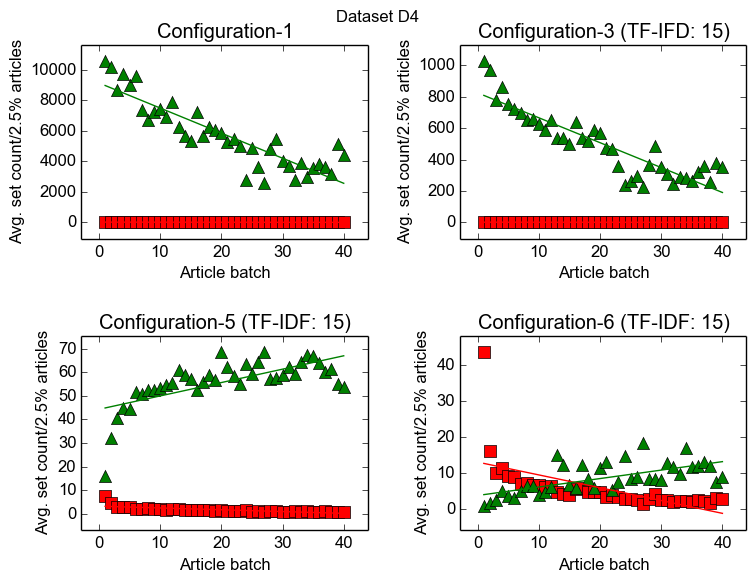
\includegraphics[scale=0.70]{images/D4-plot.png}
  \caption{Average number of new words and new pairs per batch of 2.5\% of all articles in dataset D4}
  \label{fig:setPlot4}
\end{figure}

\section{Benchmarks}
For each configuration we measured the time taken to process each of the datasets. Although each run produced the same output we performed each test 20 times to achieve more accurate benchmarks. \Cref{tab:benchmark1} shows the average time per article for different configurations. \Cref{tab:benchmark2} shows the combined average time per article for the same configurations for configurations using sub-bags and vice versa.

\begin{center}
\begin{table}
  \begin{tabular}{|l|c|}
    \hline
    Configuration & time/article (s)  \\ \hline
    Configuration-1                     & 0.3909 \\ \hline
    Configuration-2 (tfidf: 15)         & 0.2939 \\ \hline
    Configuration-4                     & 0.0533 \\ \hline
    Configuration-4 (tfidf: 15)         & 0.0488 \\ \hline
  \end{tabular}
  \caption{Average runtimes per article using different configurations}
  \label{tab:benchmark1}
\end{table}
\end{center}

\begin{center}
\begin{table}
  \begin{tabular}{|l|c|}
    \hline
    Configuration & time/article (s)             \\ \hline
    Configurations without sub-bags     & 0.3424 \\ \hline
    Configurations with sub-bags        & 0.0510 \\ \hline
  \end{tabular}
  \caption{Average runtimes per article using sub-bags or not}
  \label{tab:benchmark2}
\end{table}
\end{center}
